\section*{Results}

\subsection*{A continuous family of indistinguishable parameter sets}

Figure~\ref{fig:degeneracy}a shows two parameter quadruples related by Eq.~\eqref{eq:family} --- $(CL_d, K_p, CL_{int}, k_b) = (8.0\ \mu\text{L/min}, 5.0, 4.5\ \mu\text{L/min}, 0.0008\ \text{min}^{-1})$ and $(4.48\ \mu\text{L/min}, 1.57, 3.24\ \mu\text{L/min}, 0.003\ \text{min}^{-1})$, differing by up to 4-fold in each individual parameter --- simulated through the full nonlinear ODE system over a 33-hour incubation. The two resulting media concentration-time curves are visually superimposed throughout. Figure~\ref{fig:degeneracy}b shows the relative difference between the two curves directly: it remains below $3.9\times10^{-7}$ at every time point, consistent with the two trajectories being analytically identical and differing only at the level of numerical solver tolerance. This confirms, for a specific worked example, that the continuous equivalence family derived in Eq.~\eqref{eq:family} is not merely a formal algebraic statement but corresponds to a genuine, exact observational indistinguishability.

\begin{figure}[t]
\centering
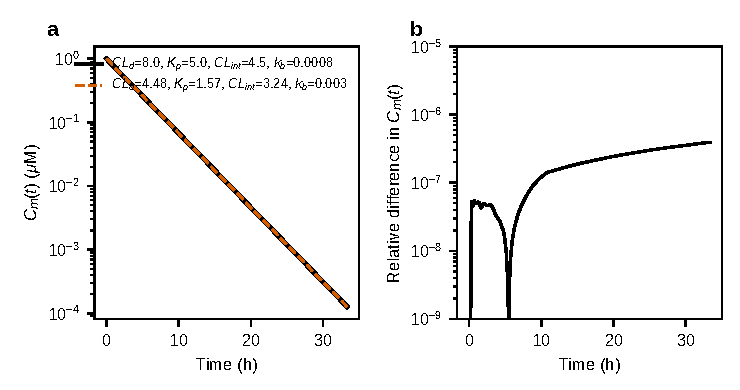
\includegraphics[width=0.75\textwidth]{figures/Fig2}
\caption{A continuous family of parameter quadruples produces identical media concentration-time data. \textbf{(a)} Media concentration $C_m(t)$ simulated from two parameter quadruples related by Eq.~\eqref{eq:family} (CN Bio hardware, constant-volume reduction). \textbf{(b)} Relative difference between the two trajectories in panel (a), remaining below $4\times10^{-7}$ throughout, consistent with numerical solver precision rather than a genuine difference in the predicted observable.}
\label{fig:degeneracy}
\end{figure}

\subsection*{Local uncertainty diagnostics are numerically unreliable near the degeneracy}

For the low-$CL_{int}$, dense-sampling scenario, the Gauss-Newton Fisher Information Matrix $J^TJ$ at the fitted optimum had a condition number of $1.38\times10^{17}$ (Fig.~\ref{fig:fim}a) --- at or beyond the limit of double-precision numerical reliability. For the high-$CL_{int}$, dense-sampling scenario, the condition number was $1.45\times10^{12}$, also indicating a numerically near-singular matrix. Correspondingly, the relative standard error of $CL_{int}$ computed via plain matrix inversion disagreed sharply with the same quantity computed via a truncated-SVD pseudoinverse on identical data: $1.40\times10^3$ (plain) versus $6.9$ (pseudoinverse) for the low-$CL_{int}$ scenario, and $2.4$ versus $0.19$ for the high-$CL_{int}$ scenario (Fig.~\ref{fig:fim}b) --- disagreements of two to three orders of magnitude from the choice of inversion algorithm alone, on the same fitted model and the same data.

\begin{figure}[t]
\centering
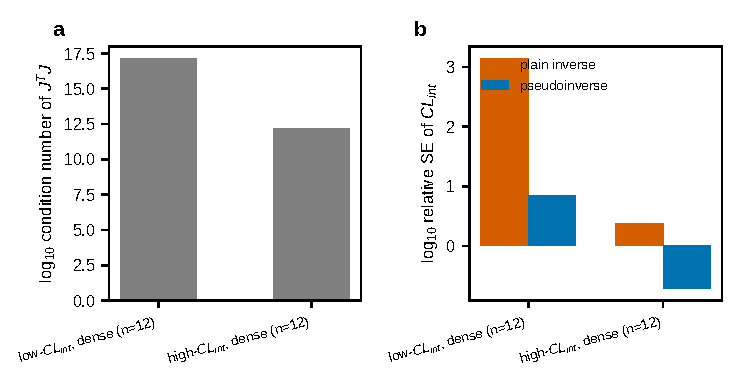
\includegraphics[width=0.75\textwidth]{figures/Fig3}
\caption{Fisher-information-based practical identifiability diagnostics are numerically unstable near the structural degeneracy. \textbf{(a)} Condition number of the Gauss-Newton Fisher Information Matrix $J^TJ$ at the fitted optimum, for two representative scenarios (dense sampling, $n=12$). \textbf{(b)} Relative standard error of $CL_{int}$ computed via plain matrix inversion versus a truncated-SVD pseudoinverse, on identical fitted data.}
\label{fig:fim}
\end{figure}

\subsection*{Single-start profile likelihood is contaminated by optimizer non-convergence}

A profile likelihood for $CL_{int}$, computed with a single optimizer start per grid point (low-$CL_{int}$, sparse sampling, $k_b$ and $e$ jointly fitted), was non-monotonic and erratic (Fig.~\ref{fig:profile}a): $\Delta$SSE remained near zero at most grid points but spiked to 0.34 at a ratio of 4.8 before falling again at larger ratios. This pattern --- a profile that is not unimodal and does not increase monotonically away from the optimum --- is inconsistent with a genuine likelihood profile and is instead diagnostic of the optimizer failing to locate the true conditional optimum at some grid points when started from a single, non-adaptive initial guess.

\subsection*{Multi-start profile likelihood: structural identifiability does not guarantee practical estimability}

Repeating the profile likelihood computation with 6 random restarts per grid point, retaining the best fit at each point, gave materially more stable profiles (Fig.~\ref{fig:profile}b). Three findings follow. First, with $k_b$ and $e$ unknown (jointly fitted) and sparse sampling, $\Delta$SSE remained near zero (all 7 scanned points inside the 95\% confidence region) across the full scanned range of $CL_{int}$ ratios (0.3$\times$ to 3.0$\times$ the true value): $CL_{int}$ is not practically constrained by this design, consistent with the structural degeneracy identified in Eq.~\eqref{eq:family}. Second, fixing $k_b$ and $e$ at their true values --- which Eq.~\eqref{eq:family} shows should render the model structurally identifiable --- did \emph{not}, in this regime, sharpen the practical identifiability of $CL_{int}$: all 7 scanned points remained inside the 95\% confidence region for sparse sampling with $k_b$, $e$ known. Third, this remained true even under dense sampling ($n=12$) with $k_b$ and $e$ known: again all 7 scanned points were inside the 95\% confidence region. In other words, removing the exact structural degeneracy by independently fixing $k_b$ and $e$ did not, by itself, translate into a practically well-constrained estimate of $CL_{int}$ in this low-clearance regime, regardless of sampling density.

\begin{figure}[t]
\centering
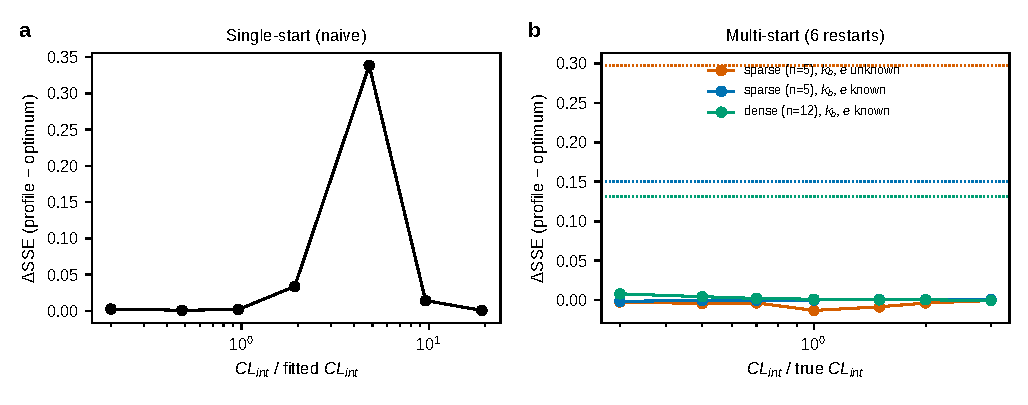
\includegraphics[width=\textwidth]{figures/Fig4}
\caption{Single-start profile likelihood is unreliable; multi-start profile likelihood reveals that resolving the structural degeneracy does not guarantee practical identifiability. \textbf{(a)} Profile likelihood for $CL_{int}$ with a single optimizer start per grid point (low-$CL_{int}$, sparse sampling, $k_b$ and $e$ jointly fitted), showing a non-monotonic, erratic profile diagnostic of optimizer non-convergence. \textbf{(b)} Profile likelihoods with 6 random restarts per grid point, for three scenarios; dotted horizontal lines mark the 95\% ($\chi^2_1$) confidence threshold for each scenario (color-matched). All three profiles remain within their respective 95\% thresholds across the full scanned range.}
\label{fig:profile}
\end{figure}

\subsection*{Summary figure}

Figure~\ref{fig:schematic} summarizes the overall argument: media-only concentration data determine three combinations of the four kinetic parameters, not the parameters themselves (panel A); the resulting one-parameter family of indistinguishable solutions collapses to a point once $k_b$ is independently measured (panel B); and structural identifiability, so achieved, is necessary but not sufficient for practical estimability, which must be assessed separately and explicitly (panel C), as demonstrated directly in Fig.~\ref{fig:profile}.

\begin{figure}[t]
\centering
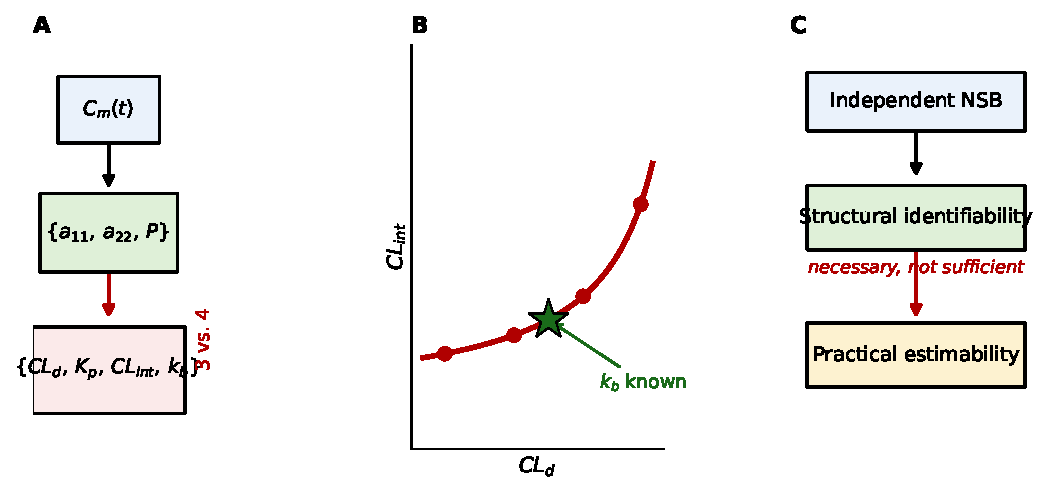
\includegraphics[width=\textwidth]{figures/Fig1}
\caption{Schematic summary. \textbf{(A)} Information bottleneck: media concentration data $C_m(t)$ determine only three combinations $\{a_{11}, a_{22}, P\}$ of the four mechanistic parameters $\{CL_d, K_p, CL_{int}, k_b\}$. \textbf{(B)} The resulting continuous equivalence family (schematic), parametrized by $k_b$; independent measurement of $k_b$ selects the true point. \textbf{(C)} Structural identifiability, once achieved, is necessary but not sufficient for practical estimability.}
\label{fig:schematic}
\end{figure}
